\documentclass{beamer}
\usepackage{graphicx} % Required for inserting images
\usepackage{amsmath}
\usepackage{tikz}
\usetikzlibrary{positioning, arrows.meta, decorations.markings, calc, intersections}
\tikzset{arrowmark/.style={postaction={decorate, decoration={markings, mark=at position #1 with {\arrow{>};}}}},
    arrowmark/.default={.5}
}


\title{Isoperimetric Inequality}
\author{Nicholas Vantine}
\date{April 2025}


\input{macros}
\input{env}

\begin{document}

\maketitle

\begin{frame}{Thanks}
\centering \Huge
\begin{itemize}
    \item \emph{DRP Organizers}
    \item \emph{Siddharth Sabharwal}
\end{itemize}
\end{frame}

\begin{frame}{The Isoperimetric Problem}
   \begin{block}{The Problem}
        Among all simple closed curves of length $\ell$ in the plane $\mathbb{R}^2$, which one encloses the largest area?
    \end{block}

    \begin{itemize}
        \item Any Guess? 
        \pause
        \item Intuition suggests the circle is optimal
        \item We'll prove this using Fourier analysis
    \end{itemize}

\begin{tikzpicture}
\centering
% First figure
\begin{scope}
    \draw[name path=mainpath] plot [smooth cycle, tension=.8] 
        coordinates {(-.5,1.5)(.5,.5)(1.5,-.5)(3,0)(4,2)(2,3)};
    \node(p1) at (2,1.5){large $A$}; 
    \node at (0,0) {$\Gamma$};
\end{scope}

% Second flatter figure
\begin{scope}[xshift=6cm]
    \draw[name path=mainpath2] plot [smooth cycle, tension=.8] 
        coordinates {(-.5,1)(.5,.2)(1.5,-.2)(3,0)(4,1)(2,1.5)};
    \node(p2) at (2,0.7){small $A$}; 
    \node at (0,0) {$\Gamma$};
\end{scope}
\end{tikzpicture}
\end{frame}

\begin{frame}{Convexity}
    \begin{definition}
        A set is convex if it contains every line segment between two points in the set.
    \end{definition}
    \begin{figure}
        \centering
        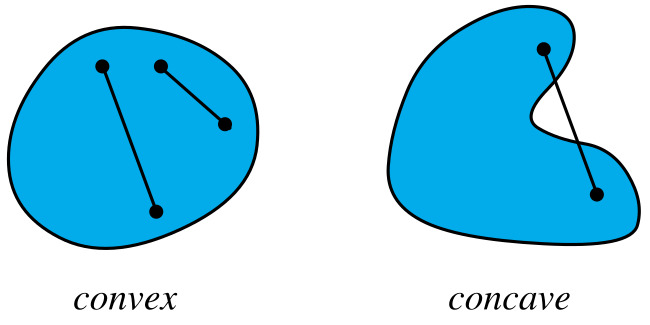
\includegraphics[width=0.5\linewidth]{convex_sets_example.jpg}
        \label{fig:enter-label}
    \end{figure}
    \begin{itemize}
        \item Think of a closed piece of string lying flat on a table
        \item making it flatter would decrease the area enclosed
        \item Want to maximize the roundness
        \item Circle is a correct guess, but how do we make it precise?
    \end{itemize}
\end{frame}

\begin{frame}{Preliminaries: Curves, Length, and Area}
    \begin{itemize}
        \item \textbf{Parametrized curve:} A mapping $\gamma: [a,b] \rightarrow \mathbb{R}^2$
        \item \textbf{Simple closed curve:} Doesn't intersect itself; endpoints coincide
            \begin{itemize}
                \item Mathematically: $\gamma(s_1) \neq \gamma(s_2)$ unless $s_1 = a$ and $s_2 = b$
                \item We require $\gamma$ to be $C^1$ with $\gamma'(s) \neq 0$ (well-defined tangent)
            \end{itemize}
        \item \textbf{Arc-length parametrization:} $|\gamma'(s)| = 1$ for all $s$
            \begin{itemize}
                \item Means $\gamma$ travels at constant speed
                \item Every curve admits this parametrization (crucial for our proof)
            \end{itemize}
        \item \textbf{Parametrization:} $\gamma(s) = (x(s), y(s))$
        \item \textbf{Length:} $\ell = \int_a^b |\gamma'(s)| ds = \int_a^b \sqrt{x'(s)^2 + y'(s)^2} \, ds$
            \begin{itemize}
                \item Independent of chosen parametrization
            \end{itemize}
        \item \textbf{Area:} $A = \frac{1}{2} \left| \int_\Gamma (x\,dy - y\,dx) \right| = \frac{1}{2} \left| \int_a^b x(s)y'(s) - y(s)x'(s) \, ds \right|$
    \end{itemize}
\end{frame}

\begin{frame}{Fourier Series}
For a function $f(\theta)$ defined on a circle (i.e., with period $2\pi$), the Fourier series is:

\begin{equation}
f(\theta) \sim \sum_{n=-\infty}^{\infty} a_n e^{in\theta}, \text{ for n}\in \Z
\end{equation}

where the Fourier coefficients $a_n$ are given by:

\begin{equation}
a_n = \frac{1}{2\pi} \int_{-\pi}^{\pi} f(\theta) e^{-in\theta} \, d\theta, \text{ for n}\in \Z
\end{equation}
\end{frame}

\begin{frame}{Properties}
    Suppose that $f$ is a continuously differentiable function on the circle. Then
    \begin{equation}
        f(\theta) \sim \sum_{n=-\infty}^{\infty} a_n e^{in\theta}
    \end{equation}
    \begin{equation}
        f'(\theta) \sim \sum_{n=-\infty}^{\infty} a_n ine^{in\theta}
    \end{equation}
    Obtained using integration by parts.
\end{frame} 

\begin{frame}{Parseval's Identity}
    Let $f$ be an integrable function on the circle with 
    \begin{equation}
        f \sim \sum_{n=-\infty}^{\infty} a_n e^{in\theta}.
    \end{equation}
    Then we have,
    \begin{equation}
        \sum_{n=-\infty}^{\infty} |a_n|^2 = \frac{1}{2\pi} \int_{0}^{2\pi} |f(\theta)|^2 d\theta
    \end{equation}
\end{frame}

\begin{frame}{Bilinear Form}
    Suppose $F$ and $G$ are integrable on the circle with 
    \begin{equation}
        F \sim \sum_{n=-\infty}^{\infty} a_n e^{in\theta} \text{ and } G \sim \sum_{n=-\infty}^{\infty} a_n e^{in\theta}
    \end{equation}
    Then
    \begin{equation}
        \frac{1}{2\pi} \int_{0}^{2\pi} F(\theta) \overline{G(\theta)} d\theta = \sum_{n=-\infty}^{\infty} a_n \overline{b_n}
    \end{equation}
\end{frame}



\section{The Isoperimetric Inequality}

\begin{frame}{The Isoperimetric Inequality}
    \begin{theorem}
        Suppose $\Gamma$ is a simple closed curve in $\mathbb{R}^2$ of length $\ell$, and let $A$ denote the area of the region enclosed by this curve. Then
        $$A \leq \frac{\ell^2}{4\pi}$$
        with equality if and only if $\Gamma$ is a circle.
    \end{theorem}
\end{frame}

\begin{frame}{Rescaling the Problem}
    \begin{itemize}
        \item By rescaling, we can set $\ell = 2\pi$
        \item Need to prove: If $\ell = 2\pi$ then $A \leq \pi$
        \item Use arc-length parametrization: $\gamma(s) = (x(s), y(s))$ with $|\gamma'(s)| = 1$
        \item So $\frac{1}{2\pi}\int_0^{2\pi} (x'(s)^2 + y'(s)^2) \, ds = 1$
    \end{itemize}
\end{frame}

\begin{frame}{Fourier Series Approach}
    \begin{itemize}
        \item Express $x(s)$ and $y(s)$ as Fourier series:
        $$x(s) \sim \sum a_n e^{ins} \quad \text{and} \quad y(s) \sim \sum b_n e^{ins}$$
        \item Then their derivatives are:
        $$x'(s) \sim \sum a_n ine^{ins} \quad \text{and} \quad y'(s) \sim \sum b_n ine^{ins}$$
        
    \end{itemize}
\end{frame}


\begin{frame}{Parseval's Identity Application}
    \begin{itemize}
        \item Unit speed curve means: $x'(s)^2 + y'(s)^2 = 1$ for all $s$
        \item Integrating over the curve:
        $$\frac{1}{2\pi}\int_0^{2\pi} (x'(s)^2 + y'(s)^2) \, ds = 1$$
        \item From Fourier derivatives:
        $$x'(s) \sim \sum_{n=-\infty}^{\infty} (in)a_n e^{ins}$$
        $$y'(s) \sim \sum_{n=-\infty}^{\infty} (in)b_n e^{ins}$$
        \item By Parseval's identity:
        $$\frac{1}{2\pi}\int_0^{2\pi} |x'(s)|^2 ds = \sum_{n=-\infty}^{\infty} |ina_n|^2$$
        $$\frac{1}{2\pi}\int_0^{2\pi} |y'(s)|^2 ds = \sum_{n=-\infty}^{\infty} |inb_n|^2$$
        \item Combining these:
        $$\sum_{n=-\infty}^{\infty} |n|^2 (|a_n|^2 + |b_n|^2) = 1$$
    \end{itemize}
\end{frame}

\begin{frame}{Parseval's Identity Application}
    \begin{itemize}
        \item Therefore we have:

        $$\frac{1}{2\pi}\int_0^{2\pi} x'(s)^2 ds + \frac{1}{2\pi}\int_0^{2\pi} y'(s)^2 \, ds = 1$$

        $$ \sum_{n=-\infty}^{\infty} |ina_n|^2 + \sum_{n=-\infty}^{\infty} |inb_n|^2 = 1$$

        $$\sum_{n=-\infty}^{\infty} (|ina_n|^2 + |inb_n|^2) = 1$$
        
        $$\sum_{n=-\infty}^{\infty} |n|^2 (|a_n|^2 + |b_n|^2) = 1$$
        
    \end{itemize}
\end{frame}

   
\begin{frame}{Bilinear Form Application}
   \begin{itemize}
   \item The complex conjugate: if $z=a+bi$, then $\overline{z} = a-bi$
   \item Recall Parseval's bilinear form:
       \begin{equation}
       \frac{1}{2\pi} \int_{0}^{2\pi} F(\theta) \overline{G(\theta)} d\theta = \sum_{n=-\infty}^{\infty} a_n \overline{b_n}
       \end{equation}
       where $F(\theta) = \sum_{n=-\infty}^{\infty} a_n e^{in\theta}$ and $G(\theta) = \sum_{n=-\infty}^{\infty} b_n e^{in\theta}$
       
   \item The area can be expressed as:
       $$A = \frac{1}{2} \left| \int_{\Gamma} (x \, dy - y \, dx) \right| = \frac{1}{2} \left| \int_{0}^{2\pi} x(s)y'(s) - y(s)x'(s) \, ds \right|$$
   
  
   \end{itemize}
\end{frame}

\begin{frame}{Billinear Form Application}
    \begin{itemize}
    \item Parseval's bilinear form:
       \begin{equation}
       \frac{1}{2\pi} \int_{0}^{2\pi} F(\theta) \overline{G(\theta)} d\theta = \sum_{n=-\infty}^{\infty} a_n \overline{b_n}
    \end{equation}
    \item Apply Parseval's identity:
       $$A = \frac{1}{2} \left| \int_{0}^{2\pi} x(s)y'(s) ds - \int_{0}^{2\pi} y(s)x'(s) \, ds \right|$$
       $$ \frac{1}{2}\left| 2\pi \sum_{n=-\infty}^{\infty}a_n \overline{inb_n} - 2\pi \sum_{n=-\infty}^{\infty} b_n \overline{ina_n}\right|$$
       $$ \pi \left| \sum_{n=-\infty}^{\infty}a_n \overline{inb_n} - b_n \overline{ina_n}\right|$$
       
       $$A = \pi \left| \sum_{n=-\infty}^{\infty} n(a_n \bar{b}_n - b_n \bar{a}_n) \right|$$
    \end{itemize}
\end{frame}
    
\begin{frame}{Proof of the Inequality}
    
    \begin{itemize}
        \item we have: $$A = \pi \left| \sum_{n=-\infty}^{\infty} n(a_n \bar{b}_n - b_n \bar{a}_n) \right|$$
        and 
         $$\sum_{n=-\infty}^{\infty} |n|^2 (|a_n|^2 + |b_n|^2) = 1$$
        \item Show that $|a_n\bar{b}_n - b_n\bar{a}_n| \leq 2|a_n||b_n| \leq |a_n|^2 + |b_n|^2$
        \item Since $|n| \leq |n|^2$:
        $$A \leq \pi \sum_{n=-\infty}^{\infty} |n|^2(|a_n|^2 + |b_n|^2) = \pi$$
    \end{itemize}
\end{frame}

\begin{frame}{The Case of Equality}
    When $A = \pi$, we must have:
    \begin{itemize}
        \item Only coefficients with $|n| \leq 1$ can be non-zero
            \begin{itemize}
                \item Since $|n| < |n|^2$ for $|n| \geq 2$, higher terms would make $A < \pi$
            \end{itemize}
            
        \item The Fourier series simplify to:
            \begin{align*}
                x(s) &= a_{-1}e^{-is} + a_0 + a_1e^{is} \\
                y(s) &= b_{-1}e^{-is} + b_0 + b_1e^{is}
            \end{align*}
            
        \item Since $x(s)$ and $y(s)$ are real-valued: $a_{-1} = \overline{a_1}$ and $b_{-1} = \overline{b_1}$
        
        \item The arc-length condition gives: $2(|a_1|^2 + |b_1|^2) = 1$
        
        \item For equality in $|a_n\overline{b}_n - b_n\overline{a}_n| \leq |a_n|^2 + |b_n|^2$:
            \begin{itemize}
                \item $|a_1| = |b_1| = \frac{1}{2}$ and $a_1 = \frac{e^{i\alpha}}{2}$, $b_1 = \frac{e^{i\beta}}{2}$
                \item $\alpha - \beta = \frac{k\pi}{2}$ where $k$ is odd
            \end{itemize}
            
        \item This gives:
            \begin{align*}
                x(s) &= a_0 + \cos(s + \alpha) \\
                y(s) &= b_0 \pm \sin(s + \alpha)
            \end{align*}
            
        \item These are exactly the parametric equations of a circle!
    \end{itemize}
\end{frame}



\begin{frame}{References}
    \begin{thebibliography}{99}
        \bibitem{book} Stein \& Shakarchi, \textit{Fourier Analysis: An Introduction}, Princeton University Press
    \end{thebibliography}
    \begin{figure}
        \centering
        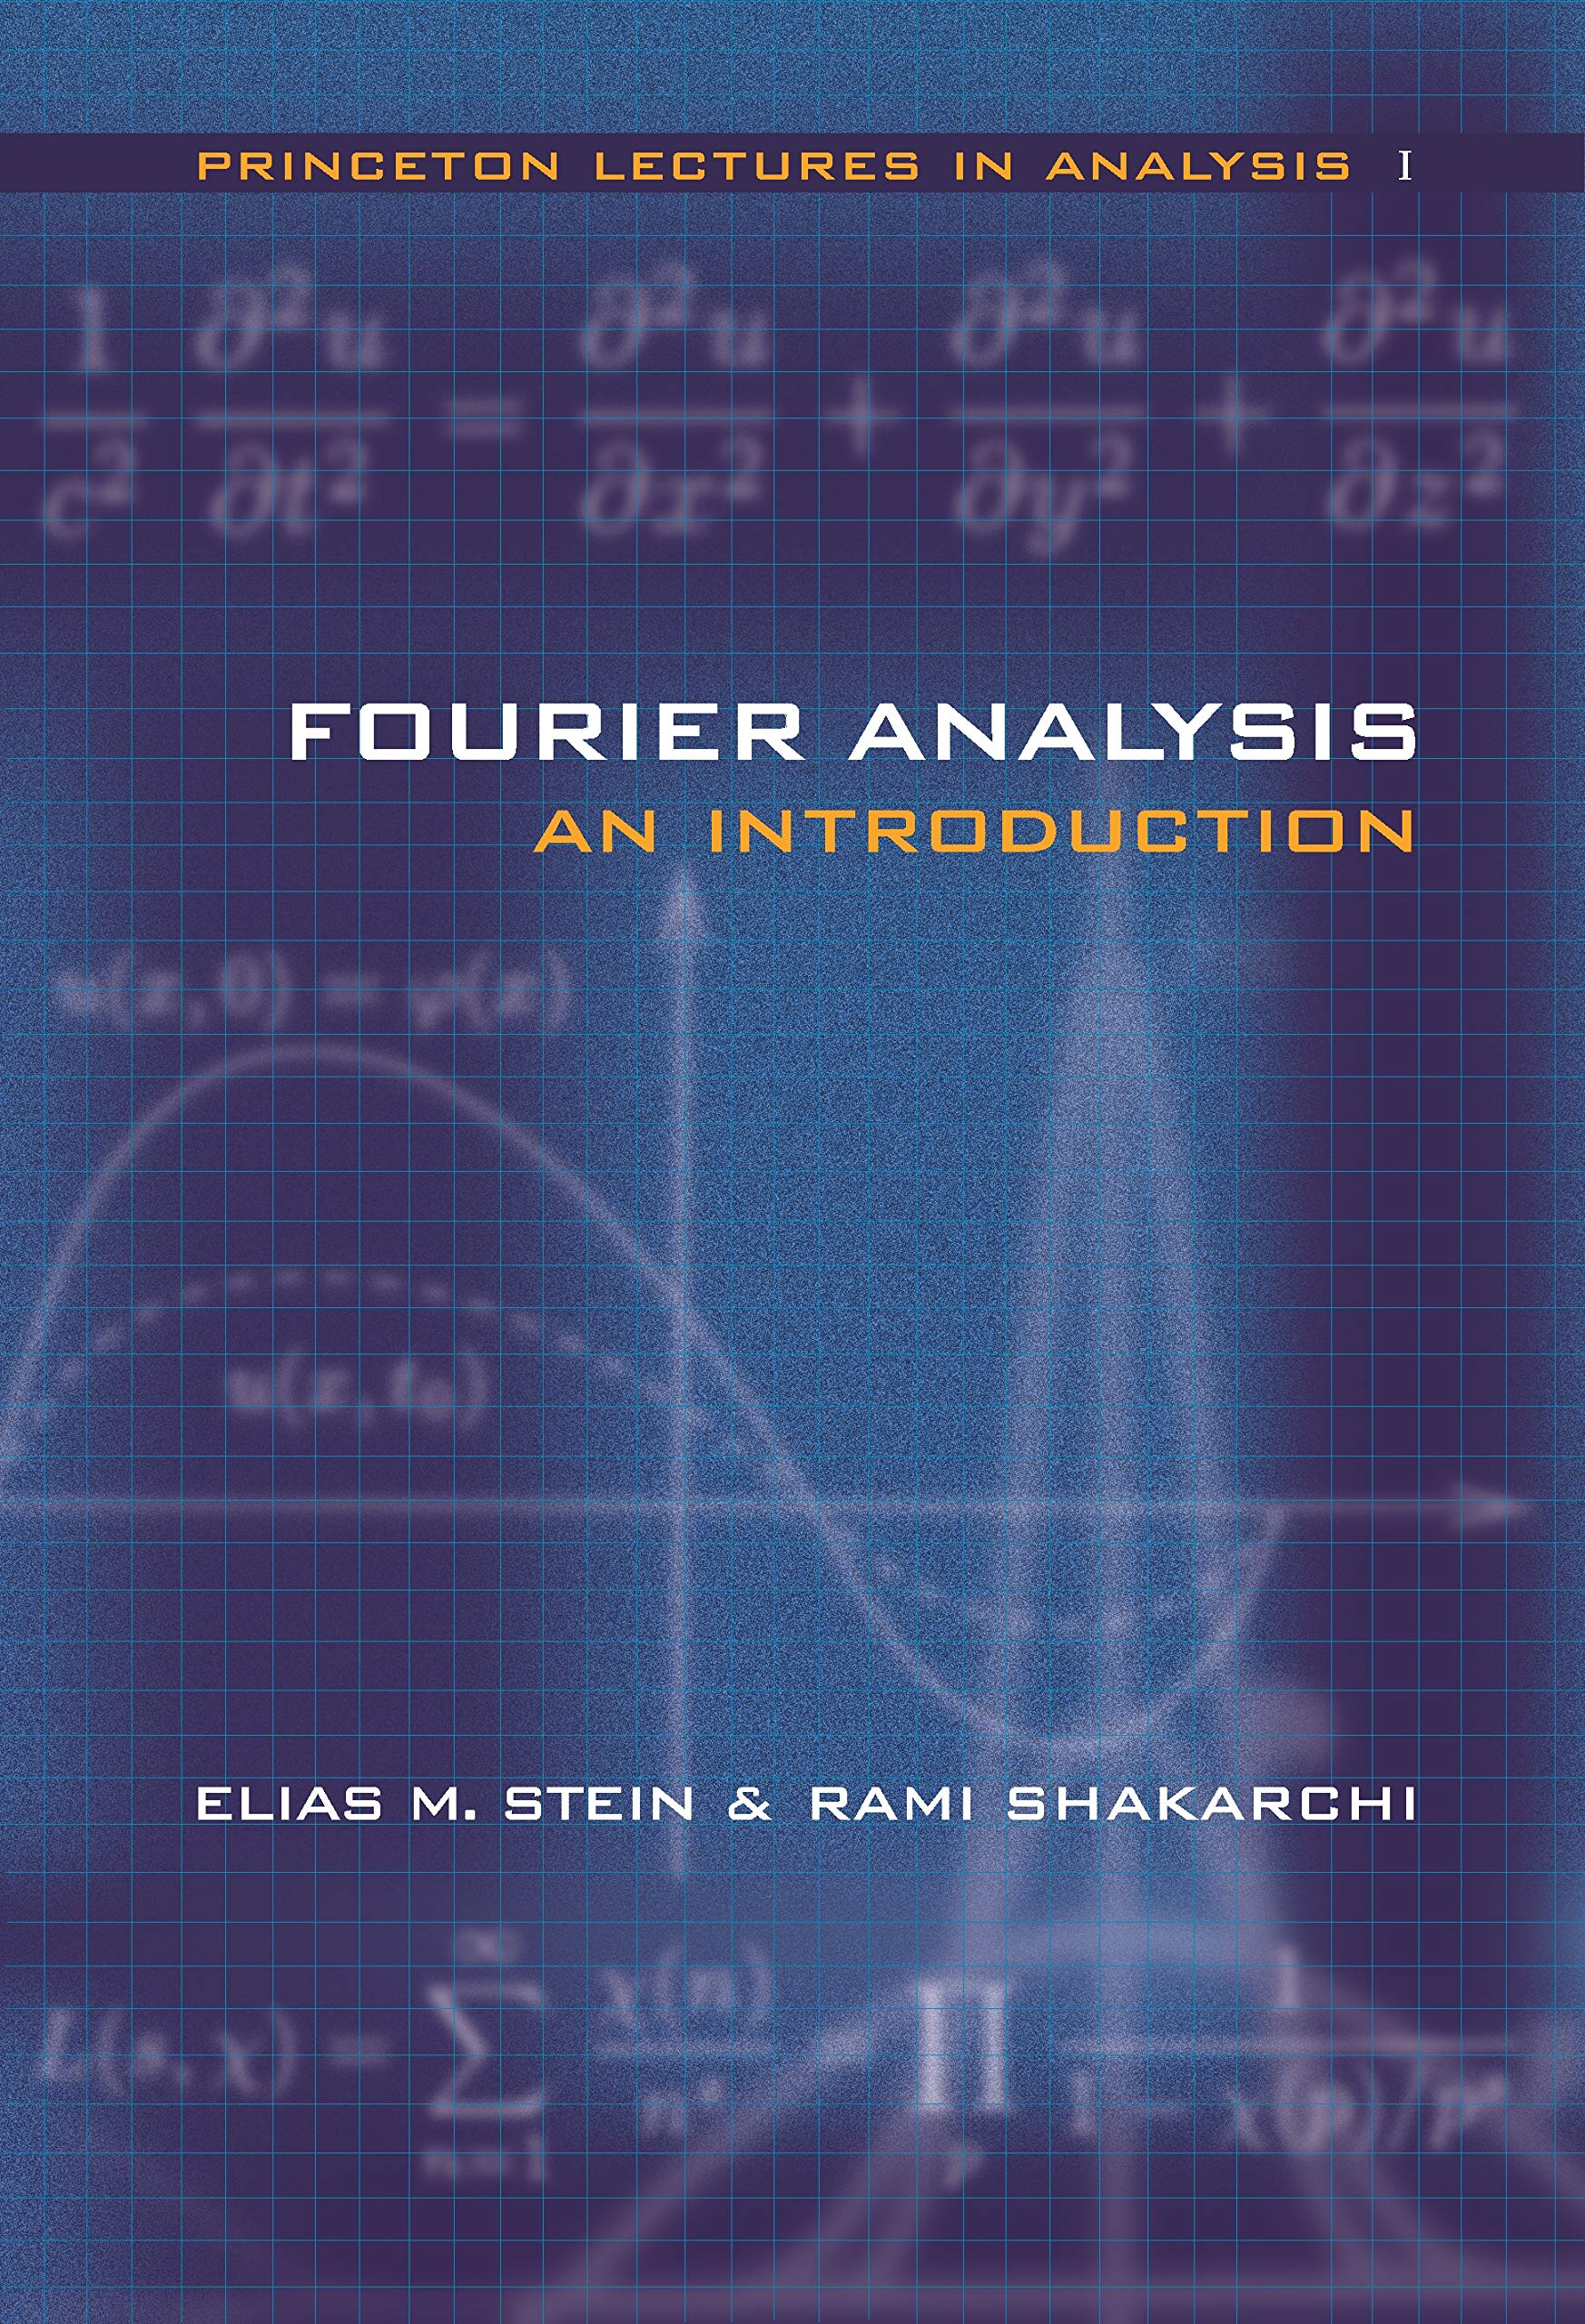
\includegraphics[width=0.4\linewidth]{book_cover.jpg}
        \label{fig:enter-label}
    \end{figure}
\end{frame}

\begin{frame}{}
  \centering \Huge
  \begin{itemize}
      \item \emph{Thanks for Listening!}
      \item \emph{Questions?}
  \end{itemize}
    
\end{frame}


\end{document}
